\documentclass[11pt,aspectratio=169]{beamer}

\usetheme[progressbar=frametitle]{metropolis}
\usepackage[italian]{babel}
\usepackage{caption}

\definecolor{myblue}{rgb}{0.19,0.55,0.91}
\usetheme[progressbar=frametitle]{metropolis}
\useoutertheme{metropolis}
\useinnertheme{metropolis}
\setbeamercolor{background canvas}{bg=white}

%\usecolortheme[named=myblue]{structure}
\setbeamercolor{frametitle}{bg=myblue}

\usepackage{appendixnumberbeamer}
\usepackage{tikz}
\usetikzlibrary{arrows}
\usepackage{booktabs}
\usepackage{verbatim}
\usepackage[scale=2]{ccicons}
\usetikzlibrary{backgrounds}
\usepackage{pgfplots}
\usepgfplotslibrary{dateplot}
\setbeamertemplate{title page}{
  \begin{minipage}[b][\paperheight]{\textwidth}
    \ifx\inserttitlegraphic\@empty\else\usebeamertemplate*{title graphic}\fi
    \vfill%
    \vspace*{20mm}
    \ifx\inserttitle\@empty\else\usebeamertemplate*{title}\fi
    \ifx\insertsubtitle\@empty\else\usebeamertemplate*{subtitle}\fi
    \usebeamertemplate*{title separator}
    \ifx\beamer@shortauthor\@empty\else\usebeamertemplate*{author}\fi
    \ifx\insertdate\@empty\else\usebeamertemplate*{date}\fi
    \ifx\insertinstitute\@empty\else\usebeamertemplate*{institute}\fi
    \vfill
    \vspace*{1mm}
  \end{minipage}
}

\setbeamertemplate{frame footer}{Andrea Carubelli}

\makeatletter
\setlength{\metropolis@progressinheadfoot@linewidth}{4pt}
\makeatother
\usepackage{xspace}
\newcommand{\themename}{\textbf{\textsc{metropolis}}\xspace}

\title{\centerline{\LARGE{Urban Stories Sharing: La app di raccolta}}}
% \subtitle{A modern beamer theme}
% \date{\today}
\date{}
\author{\textbf{Laureando:} Andrea Carubelli\newline \textbf{Matricola:} 803192 \newline \newline \textbf{Relatore:} Prof.ssa Micucci Daniela\\ \textbf{Correlatore:} Dott. Ginelli Davide}
%\institute{Università degli Studi di Milano - Bicocca}
\titlegraphic{\begin{minipage}{0.15\textwidth}
\includegraphics[height=1.5cm]{Tesi/images/logo_unimib.pdf}\end{minipage} \begin{minipage}{0.7\textwidth} \footnotesize{Università degli Studi di Milano - Bicocca \newline Dipartimento di Informatica, Sistemistica e Comunicazione \newline Corso di Laurea Triennale in Informatica} \end{minipage}\begin{minipage}{0.15\textwidth} 
\includegraphics[height=1.4cm]{Tesi/images/logo_disco.png}\end{minipage}}

\begin{document}

\maketitle


\begin{frame}{Walkability}
   Che cos'è la \textit{\textbf{walkability}}?
    
    \begin{center}\large{Il termine walkability, generalmente, indica il livello di comfort e sicurezza per i pedoni in una certa area urbana.}
    \end{center}

\end{frame}

\begin{frame}{Il contesto}
L'applicazione Android sviluppata, fa parte del progetto \textbf{Longevicity}, che studia le soluzioni per coinvolgere le persone anziane nel contesto urbano, migliorandone la qualità degli spostamenti. Il progetto è supportato dalla fondazione \textbf{Cariplo}.
    
\end{frame}

\begin{frame}{Perchè è nato il progetto?}
\begin{center}
    Migliorare la walkability di una certa area urbana attraverso storie.
\end{center}
\begin{columns}[onlytextwidth]
\begin{column}{.45\textwidth}
\begin{figure}
  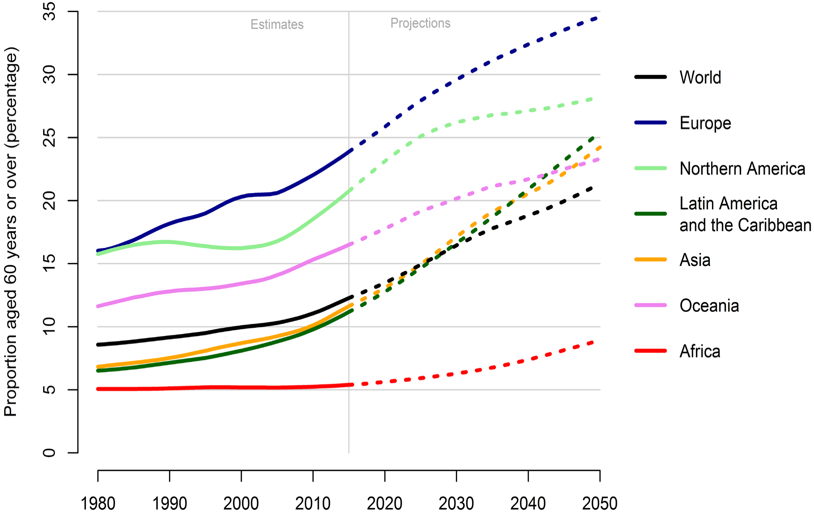
\includegraphics[scale=0.45]{Tesi/images/invecchiamento-popolazione.png}
    \captionsetup{labelformat=empty}
    \caption{\tiny{\textit{World Population Prospects: the 2017 Revision}}}
\end{figure}
\end{column}
\hfill
\begin{column}{.45\textwidth}
\begin{figure}
  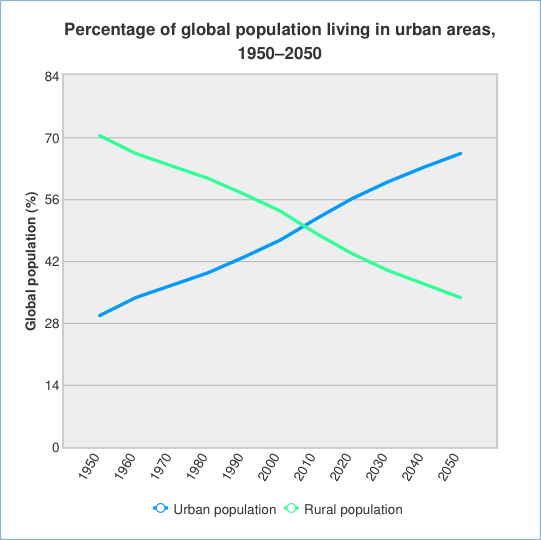
\includegraphics[scale=0.5]{Tesi/images/urbanizzazione.png}
    \captionsetup{labelformat=empty}
    \caption{\tiny{\textit{World Urbanization Prospects: the 2014 Revision}}}\hfill
\end{figure}
\end{column}
\end{columns}
\end{frame}

\begin{frame}{Il progetto}

Le principali funzioni dell'applicazione mobile sono:
\begin{itemize}
    \item Geolocalizzare gli utenti in una mappa 
    \item Condividere storie attraverso note
    \item Modificare gli elementi che caratterizzano una nota
    \item Salvare ed inviare i file multimediali, di cui sono composte le note, ad un repository centralizzato
\end{itemize}
    
\end{frame}


\begin{frame}{La mappa}

\noindent
    \begin{minipage}{0.3\textwidth}
    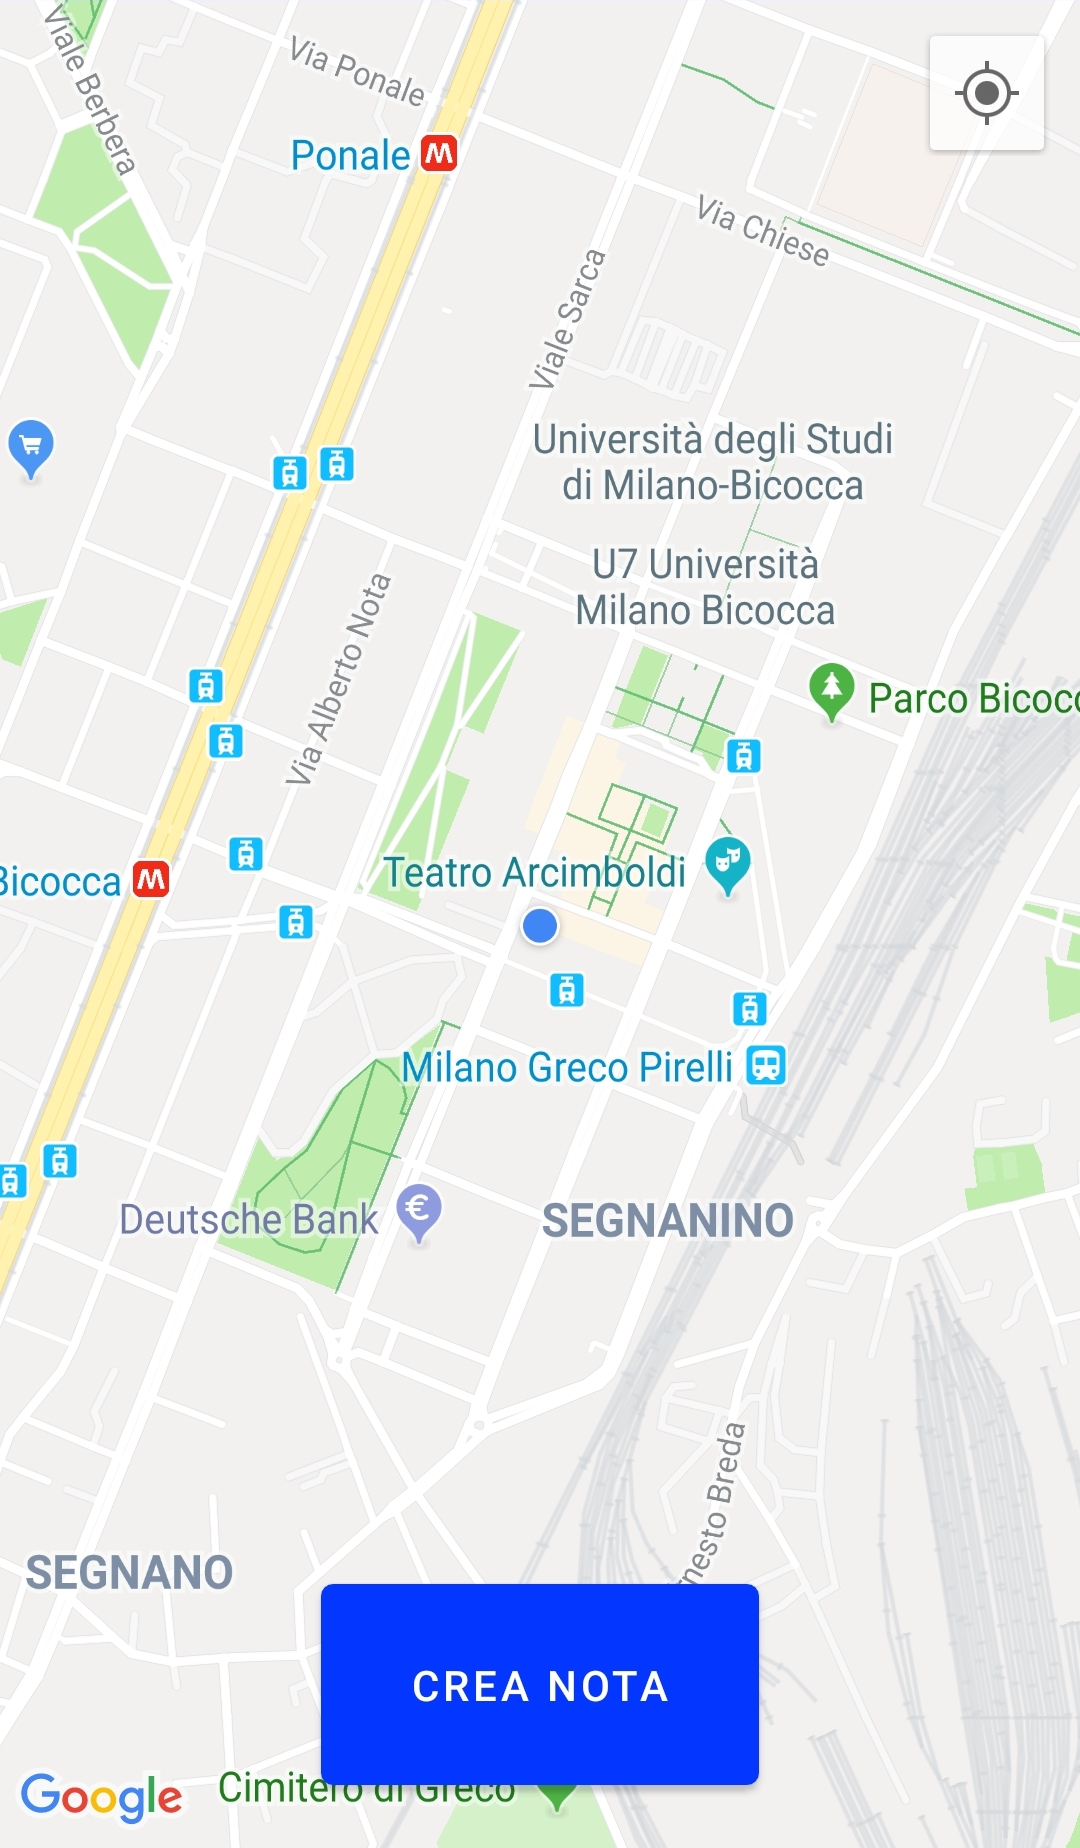
\includegraphics[scale=0.1]{Tesi/images/Mappa.jpg}
    \end{minipage}
\hfill
\begin{minipage}{0.6\textwidth}
L'utente è geolocalizzato all'interno della mappa.
\end{minipage}
\end{frame}

\begin{frame}{Homepage}
\noindent
    \begin{minipage}{0.3\textwidth}
    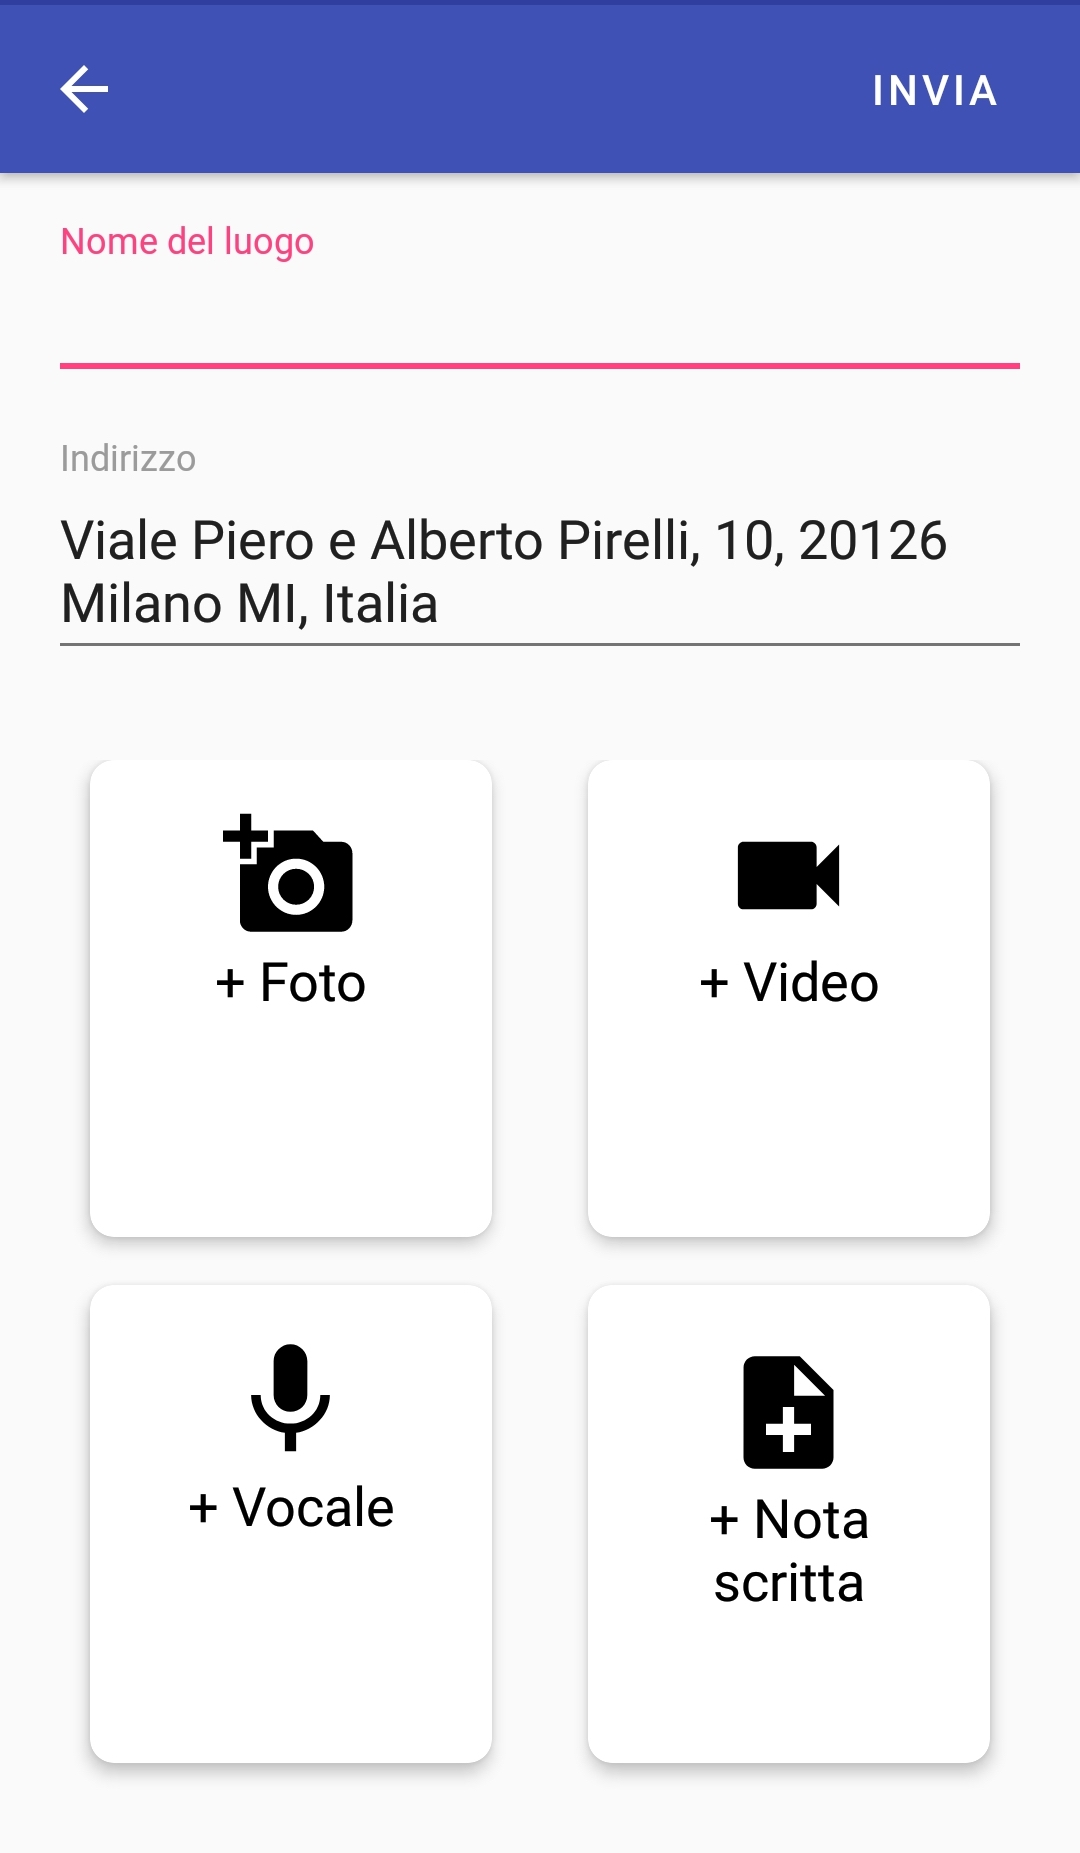
\includegraphics[scale=0.1]{Tesi/images/Homepage.jpg}
    \end{minipage}
\hfill
\begin{minipage}{0.6\textwidth}
L'utente inserirà i dati multimediali all'interno di questa pagina.
\end{minipage}
\end{frame}

\begin{frame}{Possibilità di modifica}
\noindent
    \begin{minipage}{0.3\textwidth}
    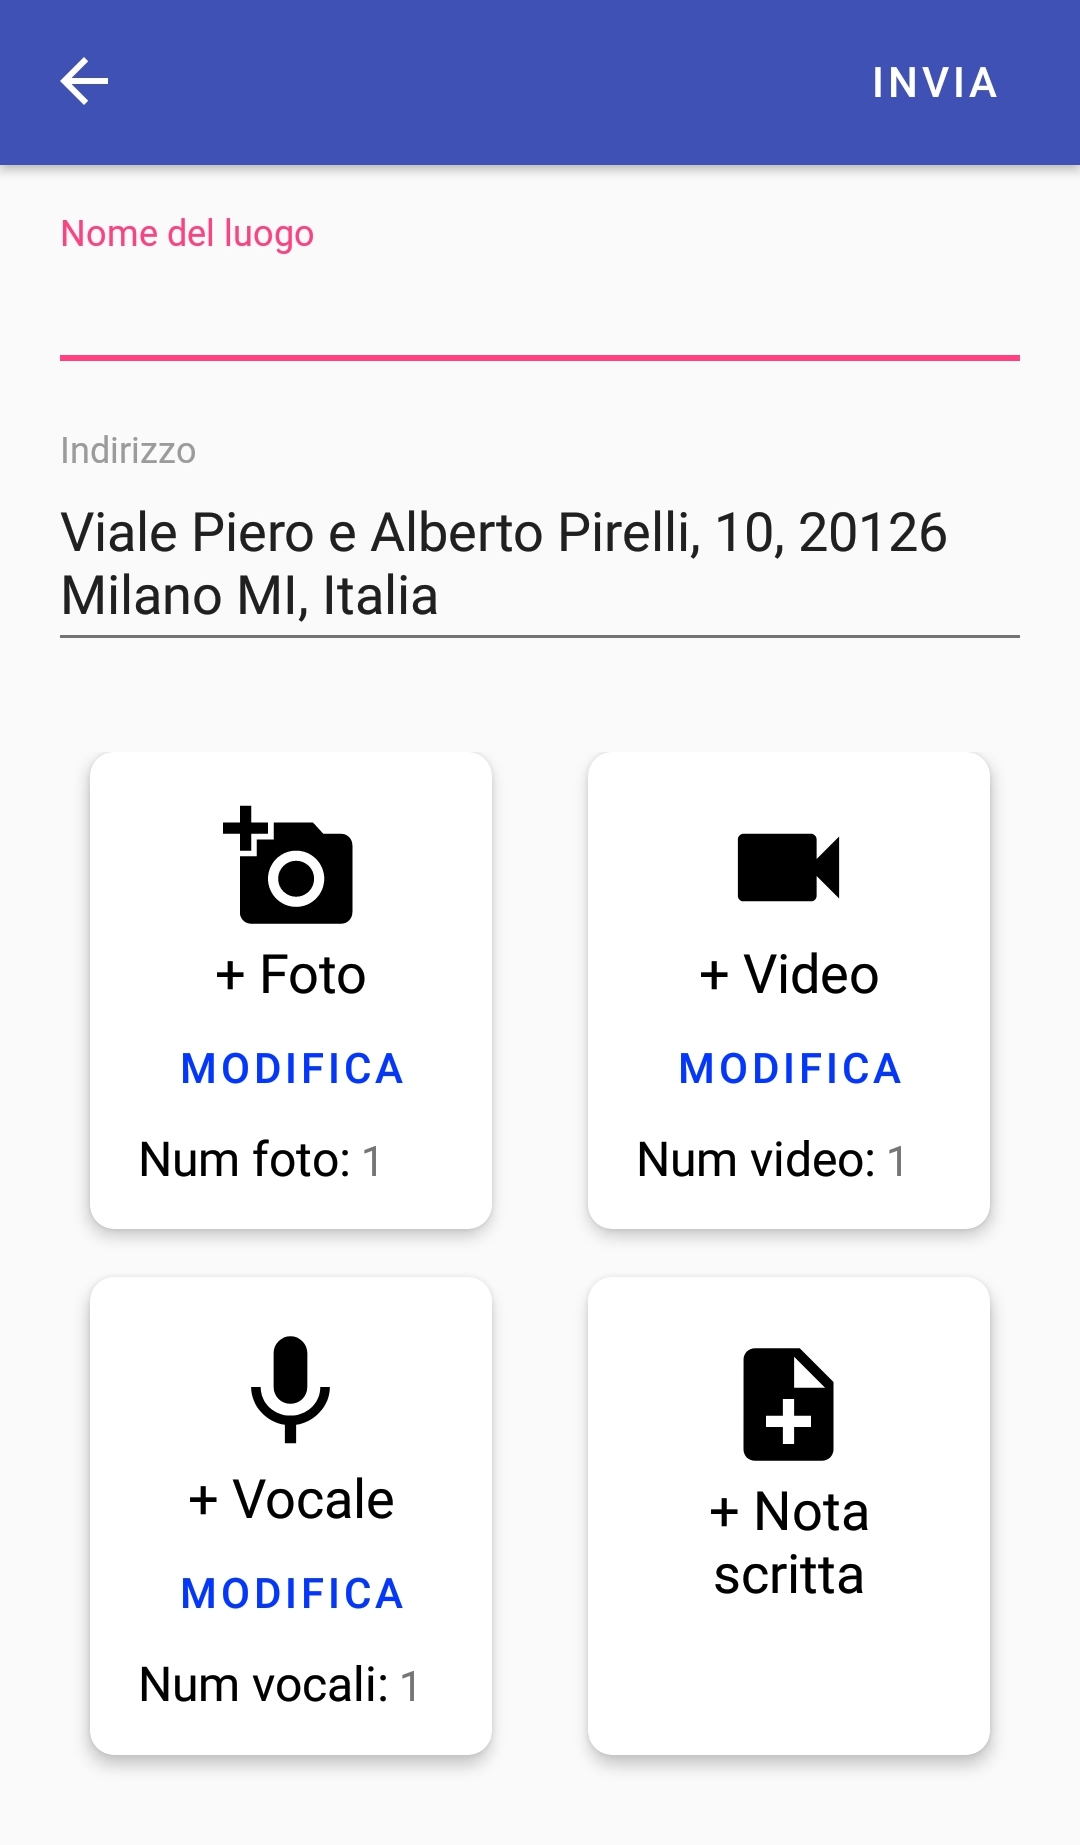
\includegraphics[scale=0.1]{Tesi/images/HomepageModifica.jpg}
    \end{minipage}
\hfill
\begin{minipage}{0.6\textwidth}
L'utente sarà anche in grado di modificare i dati precedentemente salvati.
\end{minipage}
\end{frame}

\begin{frame}{Esempio di modifica foto}
\noindent
    \begin{minipage}{0.3\textwidth}
    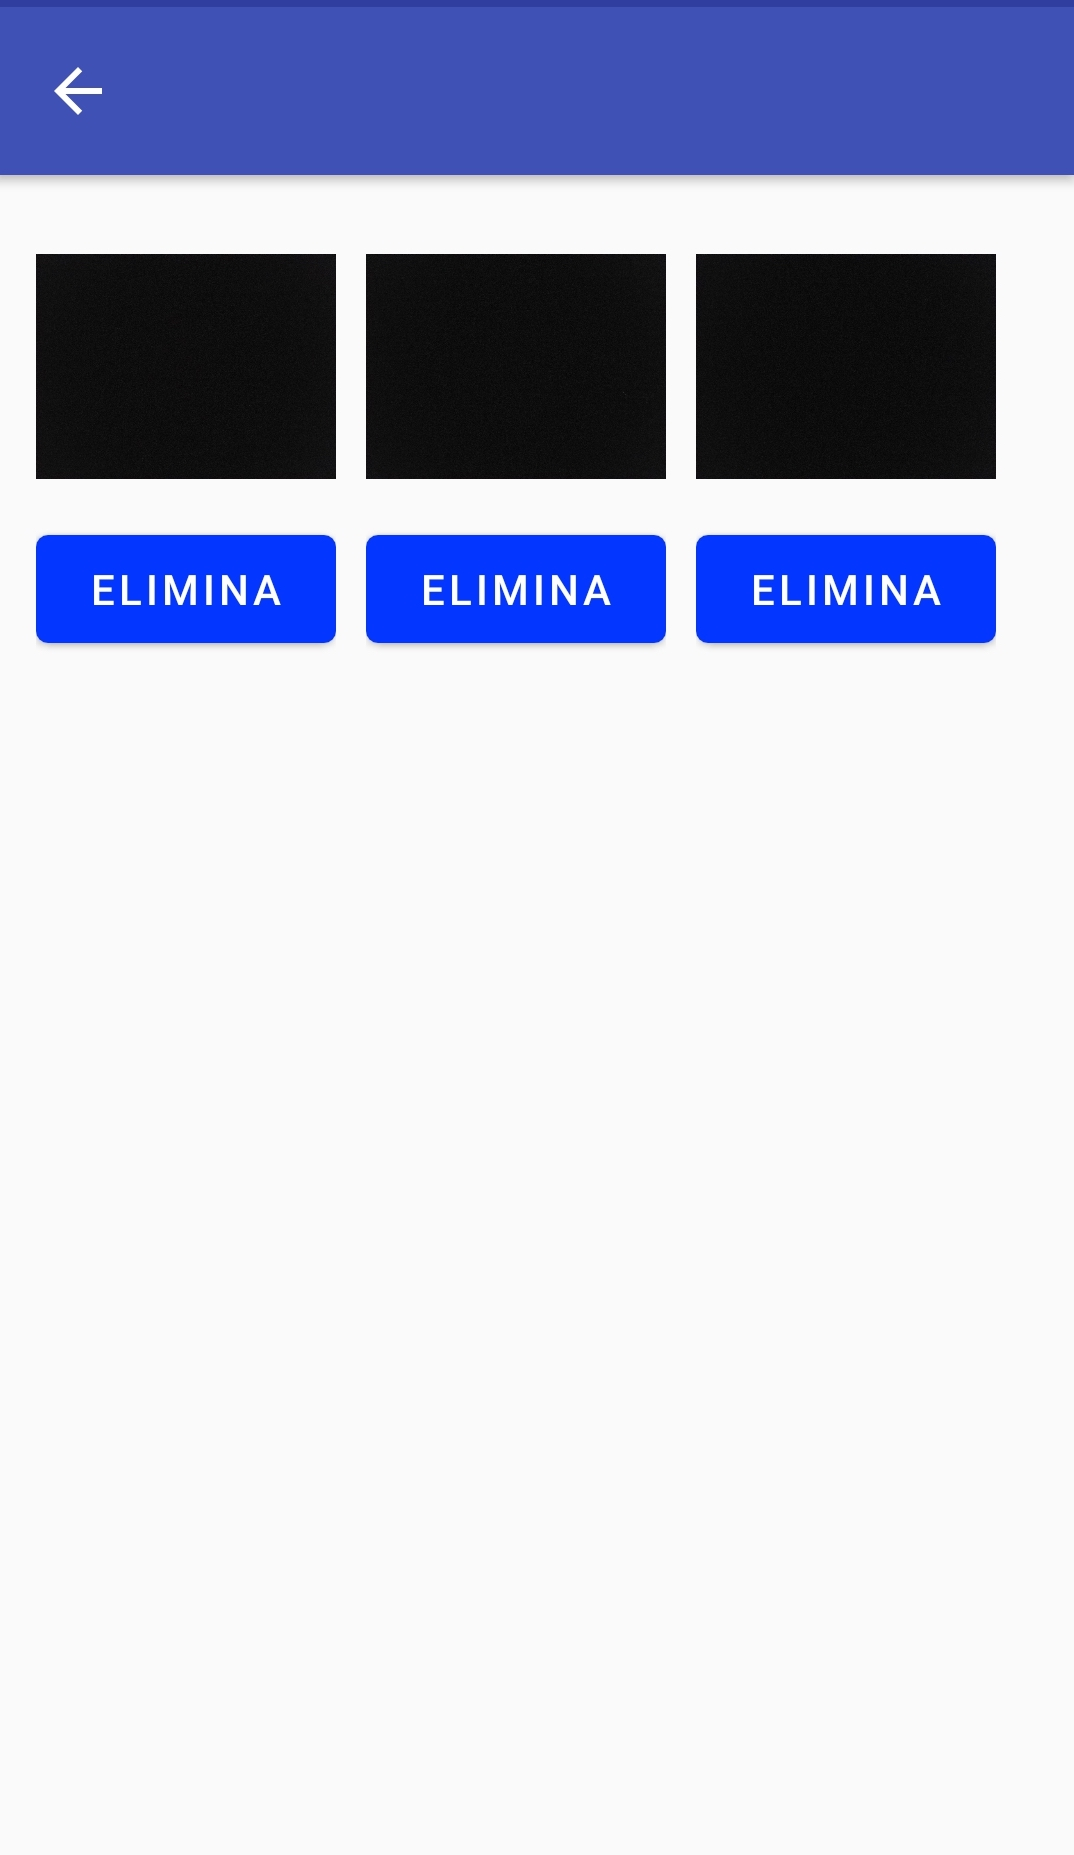
\includegraphics[scale=0.1]{Tesi/images/ModificaFoto.jpg}
    \end{minipage}
\hfill
\begin{minipage}{0.6\textwidth}
Esempio della pagina adibita alla modifica delle foto.
\end{minipage}
\end{frame}

\begin{frame}{Invio dei file}
\noindent
    \begin{minipage}{0.3\textwidth}
    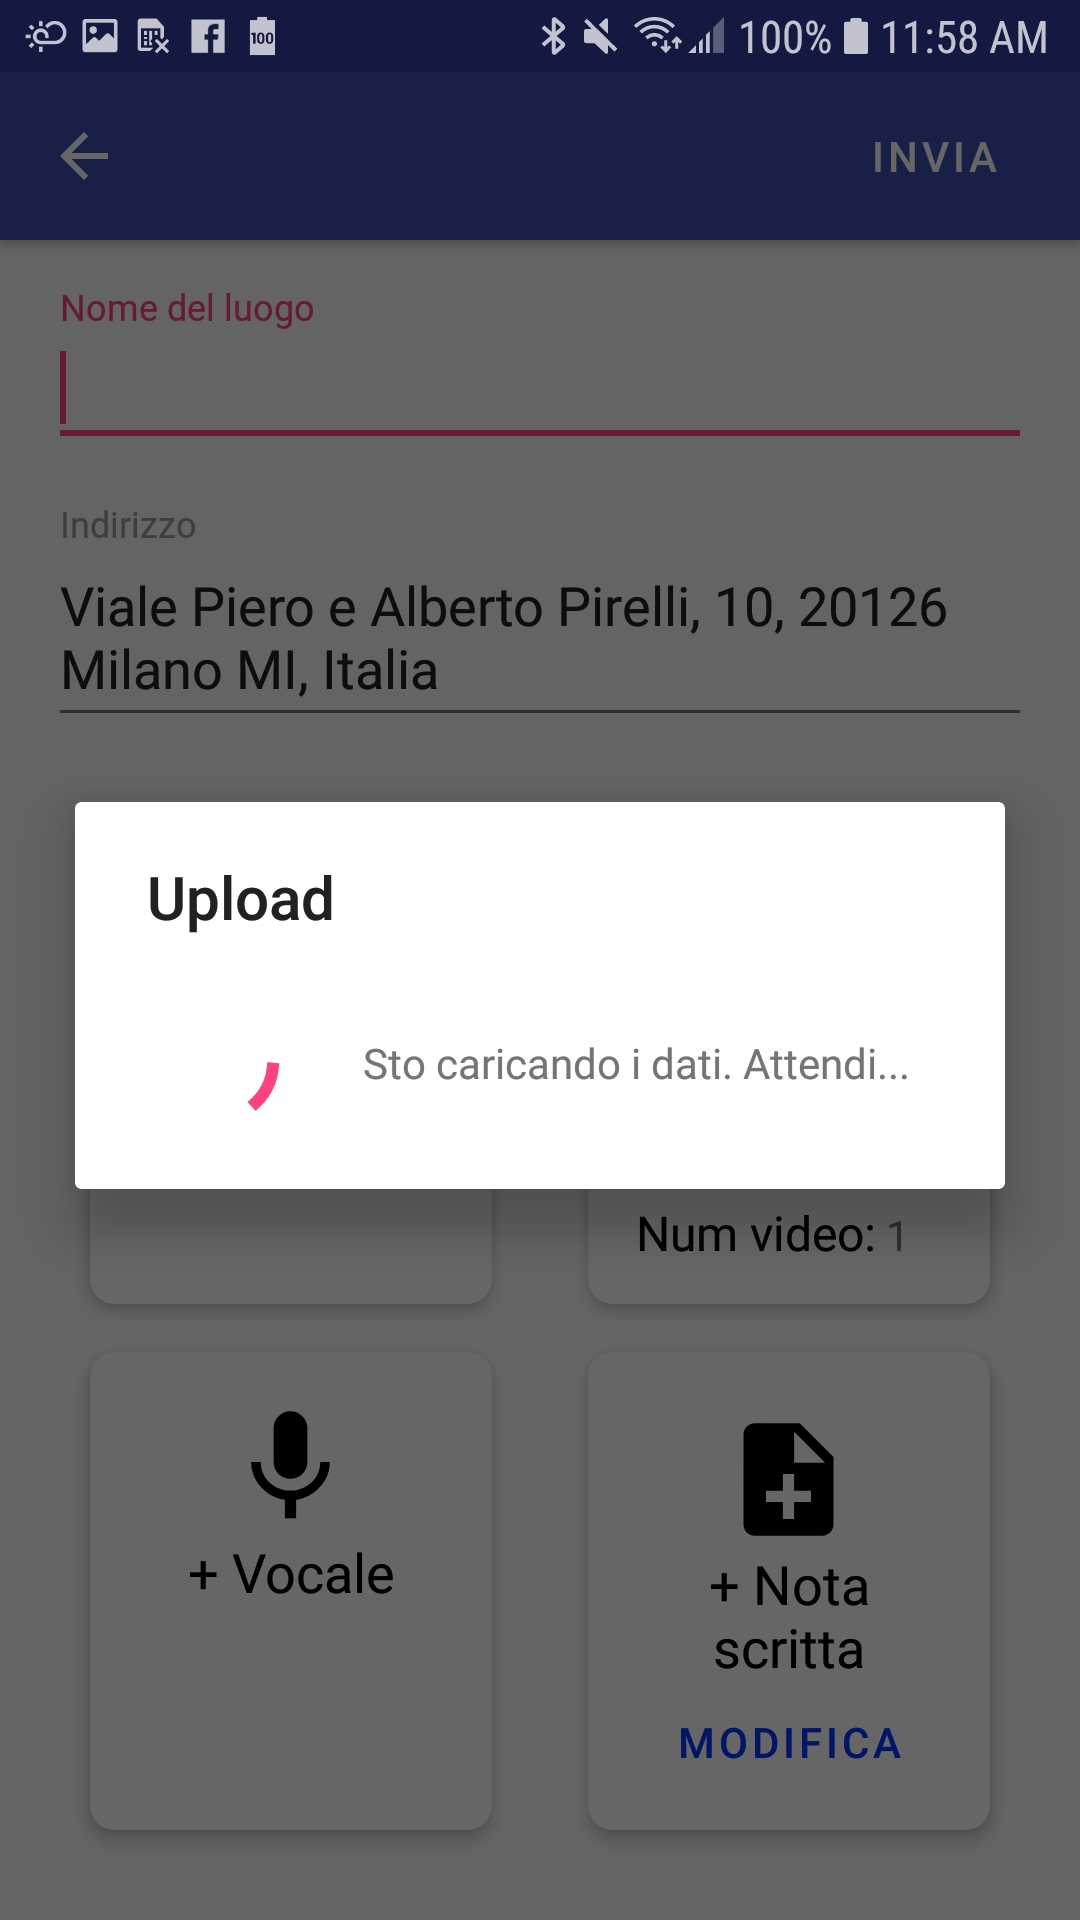
\includegraphics[scale=0.1]{Tesi/images/Progresso.jpg}
    \end{minipage}
\hfill
\begin{minipage}{0.6\textwidth}
Schiacciando il bottone "Invia", l'utente invierà i dati al database remoto.
\end{minipage}
\end{frame}

\begin{frame}{Sviluppi futuri}
    Sviluppi futuri:
    \begin{itemize}
        \item Miglioramento del design e della User Experience
        \item Cancellazione multipla degli elementi multimediali
        \item Tutorial iniziale
        \item Sistema di autenticazione
        \item Splash screen e logo app
    \end{itemize}
\end{frame}

\begin{frame}{Conclusioni}

  Il codice del mio progetto è pubblico e visibile su

  \begin{center}\url{github.com/andreacaru/urban-stories-sharing-frontend}\end{center}

  \begin{center}\LARGE{Grazie a tutti per l'attenzione}\end{center}

\end{frame}

\end{document}
